\chapter{Background}
\label{ch:background}

This chapter covers the theoretical background and related work relevant to this thesis.
The theoretical background introduces the mathematical foundations of vector representations, the Transformer architecture, and the mechanics of tool calling in large language models.
It then presents the probing methodology, the linear representation hypothesis, and the field of mechanistic interpretability, ending with representational similarity measures.
The related work section reviews the literature on tool selection, identifies the gap this thesis addresses, and explains how the experimental design follows from the documented failure modes of prior work.

\section{Theoretical Background}
\label{sec:theoretical}

This section introduces the linear algebra and neural network foundations, along with the softmax mechanics of language model output and the structure of tool-augmented prompts.
Furthermore, it presents the probing framework and its critiques, the evidence that concepts are represented as directions, and the intervention methods that turn correlational findings into causal claims.
The section closes with the similarity measures used to compare sets of representations, which are the quantities at the heart of the central research question.

\subsection{Linear Algebra Foundations}
\label{sec:linearalgebra}

Neural network states are vectors, so many measurements of models are statements about vectors.
This section fixes notation and introduces a small set of operations.
The material follows Linear Algebra and Its Applications 3rd edition by \textcite{lay2006linear}.
Proofs and a fuller treatment are found there.
\\

A vector $\mathbf{v} \in \mathbb{R}^d$ is a list of $d$ real numbers, which we write as a column:

\begin{equation}
\mathbf{v} = \begin{bmatrix} v_1 \\ v_2 \\ \vdots \\ v_d \end{bmatrix}
\label{eq:vector}
\end{equation}

In large language models, $d$ is large, typically several thousand, because each vector represents the internal state of the model at one point in its computation.
Vectors can be added and scaled.
A sum of scaled vectors is a linear combination.
The set of all linear combinations of a collection of vectors is its span.
A span forms a subspace, meaning it contains the zero vector and stays closed under addition and scalar multiplication \cite{lay2006linear}.
A set is linearly dependent when one vector in the set can be written as a linear combination of the others.
In high dimensions many directions can coexist, which is part of why models can keep many concepts in overlapping activity.
The norm of a vector, written $\lVert \mathbf{v} \rVert$, is its Euclidean length \cite[p.~331]{lay2006linear}:

\begin{equation}
\lVert \mathbf{v} \rVert = \sqrt{\sum_{i=1}^{d} v_i^2} = \sqrt{\mathbf{v}^\top \mathbf{v}}
\label{eq:norm}
\end{equation}

Two vectors can be compared by the dot product, $\mathbf{u}^\top \mathbf{v} = \sum_i u_i v_i$, which is large when the two vectors point in similar directions and zero when they are orthogonal.\footnote{Orthogonality means the vectors meet at a right angle. In high-dimensional spaces, most pairs of unrelated vectors are nearly orthogonal, so a dot product near zero is the default, and a large one is informative.}
\\

A common comparison of hidden states is cosine similarity, the cosine of the angle between two vectors \cite[p.~335]{lay2006linear}:

\begin{equation}
\cos(\mathbf{u}, \mathbf{v}) = \frac{\mathbf{u}^\top \mathbf{v}}{\lVert \mathbf{u} \rVert \, \lVert \mathbf{v} \rVert}
\label{eq:cosine}
\end{equation}

Cosine similarity ranges from $-1$ to $1$ and ignores the length of the vectors, which makes it the standard measure of directional agreement between hidden states.
A value near $1$ means the two states point in the same direction, and a value near $0$ means they are unrelated.
The dot product also defines a projection.
The scalar projection of $\mathbf{v}$ onto a unit vector $\mathbf{u}$ is $\mathbf{u}^\top \mathbf{v}$.
It gives the signed length of $\mathbf{v}$ along $\mathbf{u}$.
Every vector can be split into a part along $\mathbf{u}$ and a part orthogonal to $\mathbf{u}$.
This orthogonal decomposition underlies readings where one direction is added or removed while the rest is left unchanged \cite{lay2006linear}.
The Cauchy Schwarz inequality bounds the dot product by the product of the norms, with equality only when the vectors point in the same or opposite directions.
Cosine similarity is the normalized form of that bound.
\Cref{fig:cosine} illustrates the geometric relationship between the dot product, the angle, and the cosine.

\begin{figure}[htbp]
\centering
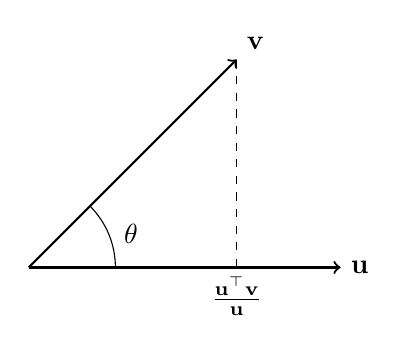
\begin{tikzpicture}[scale=2.2]
  \draw[->, thick] (0,0) -- (1.8,0) node[right] {$\mathbf{u}$};
  \draw[->, thick] (0,0) -- (1.2,1.2) node[above right] {$\mathbf{v}$};
  \draw (0.5,0) arc (0:45:0.5) node[midway, right, xshift=2pt] {$\theta$};
  \draw[dashed] (1.2,1.2) -- (1.2,0) node[below] {$\frac{\mathbf{u}^\top \mathbf{v}}{\lVert \mathbf{u} \rVert}$};
\end{tikzpicture}
\caption{Two vectors $\mathbf{u}$ and $\mathbf{v}$ with angle $\theta$ between them. The cosine similarity of \Cref{eq:cosine} is $\cos\theta$, which equals the length of the projection of $\mathbf{v}$ onto $\mathbf{u}$ when $\mathbf{u}$ has unit length. (Preliminary figure.)}
\label{fig:cosine}
\end{figure}

A linear map from $\mathbb{R}^d$ to $\mathbb{R}^k$ is a matrix $W \in \mathbb{R}^{k \times d}$ acting by matrix multiplication, $\mathbf{v} \mapsto W\mathbf{v}$.
The product $W\mathbf{v}$ is a linear combination of the columns of $W$, weighted by the entries of $\mathbf{v}$ \cite{lay2006linear}.
The transpose $W^\top$ swaps rows and columns, so $\mathbf{u}^\top \mathbf{v}$ can be read as a one row matrix applied to a column vector.
A linear classifier is a linear map followed by a decision rule.
For binary classification, the classifier computes

\begin{equation}
f(\mathbf{v}) = \mathbf{w}^\top \mathbf{v} + b
\label{eq:linearclassifier}
\end{equation}

for a learned weight vector $\mathbf{w}$ and bias $b$, and predicts one class when $f(\mathbf{v}) > 0$ and the other when $f(\mathbf{v}) < 0$.
The set of points where $\mathbf{w}^\top \mathbf{v} + b = 0$ is a hyperplane, a flat decision boundary that splits the space in two.
A pair of groups is called linearly separable when some hyperplane separates them, and the accuracy of the best such hyperplane is a working measure of how distinguishable two groups are.
\Cref{fig:separability} shows two cases side by side.

\begin{figure}[htbp]
\centering
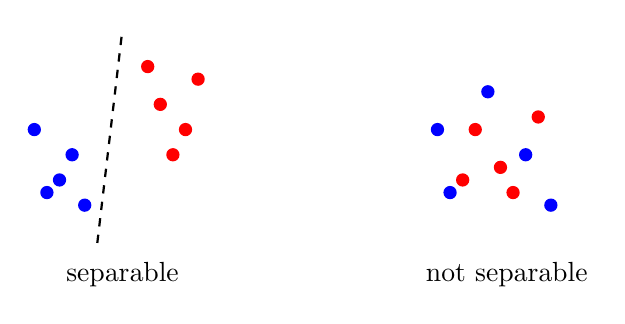
\begin{tikzpicture}[scale=1.6]
  % Left: separable
  \begin{scope}
    \foreach \p in {(0.3,0.4),(0.5,0.7),(0.2,0.9),(0.6,0.3),(0.4,0.5)} \fill[blue] \p circle (1.5pt);
    \foreach \p in {(1.2,1.1),(1.4,0.9),(1.1,1.4),(1.5,1.3),(1.3,0.7)} \fill[red] \p circle (1.5pt);
    \draw[thick, dashed] (0.7,0) -- (0.9,1.7);
    \node at (0.9,-0.25) {separable};
  \end{scope}
  % Right: not separable
  \begin{scope}[xshift=3.2cm]
    \foreach \p in {(0.3,0.4),(0.9,0.7),(0.2,0.9),(1.1,0.3),(0.6,1.2)} \fill[blue] \p circle (1.5pt);
    \foreach \p in {(0.7,0.6),(0.5,0.9),(1.0,1.0),(0.8,0.4),(0.4,0.5)} \fill[red] \p circle (1.5pt);
    \node at (0.75,-0.25) {not separable};
  \end{scope}
\end{tikzpicture}
\caption{Left: two groups of points that a hyperplane (dashed line) can separate. Right: two groups that no hyperplane can separate. Probe accuracy measures which case holds, and how close points sit to the boundary. (Preliminary figure.)}
\label{fig:separability}
\end{figure}

A final concept is the mean difference direction.
The difference between two group means, normalized to unit length, defines a direction that points from the center of group $A$ to the center of group $B$ \cite[p.~3]{wu2026linearly}.

\begin{equation}
\mathbf{d}_{A \to B} = \frac{\bar{\mathbf{h}}_B - \bar{\mathbf{h}}_A}{\lVert \bar{\mathbf{h}}_B - \bar{\mathbf{h}}_A \rVert}
\label{eq:meandiff}
\end{equation}

This mean-difference direction is the simplest summary of how two groups differ, and it appears in later sections as the steering vector of \textcite{wu2026linearly}, the function vector of \textcite{todd2024function}, and the truth direction of \textcite{marks2024geometry}.

\subsection{Neural Networks and the Transformer}
\label{sec:transformer}

A neural network is a function built by composing simple layers.
Each layer applies a linear map followed by a fixed nonlinear function, and the stack of layers maps an input to an output through a sequence of intermediate vectors.
The intermediate vectors are called activations or hidden states.
\\

Modern language models are built from the Transformer architecture \cite{vaswani2017attention}.
A Transformer language model processes a sequence of tokens, where a token is a unit of text such as a word or word fragment.\footnote{For example, the word ``unhappiness'' might be split into the tokens ``un'', ``happi'', and ``ness''. Tokenization matters for tool names because two names that share a token prefix, such as \texttt{get\_weather} and \texttt{get\_news}, begin with the same internal representation, which can blur their separation.}
Each token is first converted to a vector by an embedding table, a matrix $E \in \mathbb{R}^{|V| \times d}$ whose rows are the learned vectors of each vocabulary item.
The model then passes the sequence through a stack of identical blocks.
Each block has two parts.
The first is self-attention, which lets every token collect information from every earlier token by computing a weighted average of their values, with the weights set by how well each earlier token's key matches the current token's query \cite[p.~4]{vaswani2017attention}:

\begin{equation}
\mathrm{Attention}(Q, K, V) = \mathrm{softmax}\!\left(\frac{QK^\top}{\sqrt{d_k}}\right) V
\label{eq:attention}
\end{equation}

Here $Q$, $K$, and $V$ are matrices of query, key, and value vectors, all linear projections of the block's input, and the division by $\sqrt{d_k}$ keeps the dot products at a scale where the softmax has useful gradients \cite[p.~4]{vaswani2017attention}.
The second part is a feed-forward network applied to each position independently \cite[p.~5]{vaswani2017attention}:

\begin{equation}
\mathrm{FFN}(\mathbf{x}) = \max(0, \mathbf{x}W_1 + \mathbf{b}_1) W_2 + \mathbf{b}_2
\label{eq:ffn}
\end{equation}

This shows the original form with ReLU.
Modern instruction tuned models often use gated variants such as SwiGLU, while the residual stream reading stays the same.

Around both parts, the block uses a residual connection, meaning the input to the part is added to its output.
\Cref{fig:transformer} shows the structure of one block and how the residual stream accumulates.

\begin{figure}[htbp]
\centering
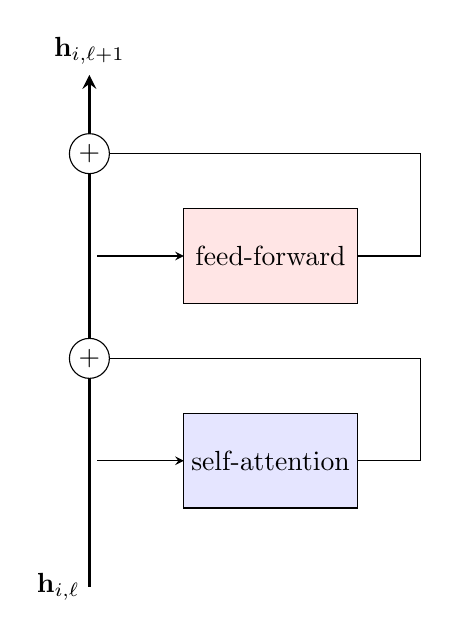
\begin{tikzpicture}[scale=1.0, >=stealth]
  % Residual stream
  \draw[->, very thick] (0,0) -- (0,6.5) node[above] {$\mathbf{h}_{i,\ell+1}$};
  \node[left] at (0,0) {$\mathbf{h}_{i,\ell}$};
  % Attention block
  \draw[fill=blue!10] (1.2,1.0) rectangle (3.4,2.2) node[midway] {self-attention};
  \draw[->] (0.1,1.6) -- (1.2,1.6);
  \draw[->] (3.4,1.6) -- (4.2,1.6) -- (4.2,2.9) -- (0.1,2.9);
  \node[circle, draw, fill=white, inner sep=1.5pt] at (0,2.9) {$+$};
  % FFN block
  \draw[fill=red!10] (1.2,3.6) rectangle (3.4,4.8) node[midway] {feed-forward};
  \draw[->] (0.1,4.2) -- (1.2,4.2);
  \draw[->] (3.4,4.2) -- (4.2,4.2) -- (4.2,5.5) -- (0.1,5.5);
  \node[circle, draw, fill=white, inner sep=1.5pt] at (0,5.5) {$+$};
\end{tikzpicture}
\caption{One Transformer block. The residual stream (vertical arrow) carries the hidden state upward, and each part of the block reads from it and adds its contribution back. The hidden state at any layer is the running sum of all earlier contributions. (Preliminary figure.)}
\label{fig:transformer}
\end{figure}

The residual connection has a useful consequence.
Because each block only adds to what came before, the hidden state at any layer can be read as a running sum of contributions from every earlier block.
This sum is called the residual stream.
Following \textcite{todd2024function}, we write the hidden state at layer $\ell$ and token position $i$ as $\mathbf{h}_{i,\ell} \in \mathbb{R}^d$, and the residual-stream view treats the model's computation as information being written into and read from this stream by each block in turn.
Formally, each layer updates the stream by \cite[p.~3]{todd2024function}

\begin{equation}
\mathbf{h}_{i,\ell} = \mathbf{h}_{i,\ell-1} + \mathbf{m}_{i,\ell} + \sum_{j=1}^{J} \mathbf{a}_{i,\ell j}
\label{eq:residual}
\end{equation}

where $\mathbf{m}_{i,\ell}$ is the feed-forward output and $\mathbf{a}_{i,\ell j}$ is the output of the $j$-th attention head, projected back into the stream.
After the final layer, the hidden state at the last position is mapped to a distribution over the vocabulary by a linear map called the unembedding, followed by a softmax.
\\

Two properties of this architecture are important.
First, the hidden state at the last token of the prompt, just before the model generates its answer, is the point where all information the model will use is already present.
The probes discussed in \cref{sec:probing} read from that position.
Second, because the unembedding is linear, the model has an architectural reason to keep the identities of different outputs pointing in distinguishable directions, a point \cref{sec:linearrep} returns to.

\subsection{Large Language Models and Tool Use}
\label{sec:llmtools}

A large language model is a Transformer trained to predict the next token.
Given a context $\mathbf{x}$, the probability distribution over the next token $y$ defined by the model can be expressed as follows \cite[p.~2]{park2024linear}:

\begin{equation}
P(y \mid \mathbf{x}) = \frac{\exp(\boldsymbol{\lambda}(\mathbf{x})^\top \boldsymbol{\gamma}(y))}{\sum_{y'} \exp(\boldsymbol{\lambda}(\mathbf{x})^\top \boldsymbol{\gamma}(y'))}
\label{eq:softmax}
\end{equation}

where $\boldsymbol{\lambda}(\mathbf{x})$ is the final hidden state of the context and $\boldsymbol{\gamma}(y)$ is the unembedding vector of token $y$.
The numerator values $\boldsymbol{\lambda}(\mathbf{x})^\top \boldsymbol{\gamma}(y)$ before normalization are called logits, and the softmax turns them into a proper probability distribution.\footnote{The softmax is monotone in the logit, so the most likely token is simply the one with the largest logit. Probability mass is a richer signal than the argmax choice, because a model that places 45\% of its mass on the wrong tool is confusable even when the top-ranked token happens to be the right one.}
Text is generated by sampling from this distribution repeatedly, each time appending the new token to the context.
Two common decoding choices are greedy decoding and temperature sampling.
Greedy decoding always takes the most likely token, and temperature rescales the distribution before sampling, with temperature zero being another name for greedy decoding.
After pretraining on raw text, models are instruction-tuned to follow commands and produce structured outputs, and it is instruction tuning that makes reliable tool calling possible \cite{schick2023toolformer}.
\\

Tool use turns the model from a text generator into an agent.
In the standard design, the prompt contains a system message, a list of tool specifications, and the user query.
Each specification consists of a name, a natural language description, and a parameter schema describing the arguments the tool accepts.
The model responds with a structured object, usually JSON, naming a tool and supplying its arguments.
A surrounding program then executes the call and feeds the result back to the model.
Benchmarks such as Gorilla \cite{patil2023gorilla}, ToolLLM \cite{qin2023toolllm}, and the Berkeley Function Calling Leaderboard \cite{yan2024bfcl} evaluate how accurately models perform this selection and formatting.
\\

The decision happens at a precise point in this pipeline.
When the model finishes reading the prompt and begins to generate the tool name, the final hidden state of the prompt holds whatever the model uses to make that choice.
The probability mass over candidate tool names at that point forms the tool choice distribution.
The hidden state and the distribution describe the same decision from two sides, one internal and one behavioral.

\subsection{Probing Internal Representations}
\label{sec:probing}

Given a trained model, a probe is a small classifier trained to predict some property from the model's hidden states.
The idea originates with \textcite{alain2016understanding}, who trained linear classifiers on the intermediate layers of image models and found that linear separability increases monotonically with depth.
The logic is that if a simple classifier can read a property out of a hidden state, then the representation contains that property in an accessible form.
\textcite{hewitt2019structural} extended this from scalar properties to structure, showing that the syntax trees of sentences can be recovered from word representations through a linear transformation under which squared distances encode tree distance.
\Cref{fig:probing} shows the basic setup.

\begin{figure}[htbp]
\centering
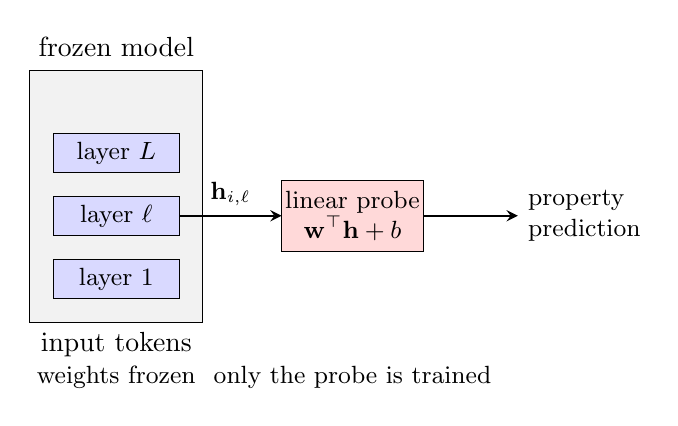
\begin{tikzpicture}[scale=1.0, >=stealth]
  % Frozen model
  \draw[fill=gray!10] (0,0) rectangle (2.2,3.2);
  \node at (1.1,3.5) {frozen model};
  \draw[fill=blue!15] (0.3,0.3) rectangle (1.9,0.8) node[midway, font=\small] {layer 1};
  \draw[fill=blue!15] (0.3,1.1) rectangle (1.9,1.6) node[midway, font=\small] {layer $\ell$};
  \draw[fill=blue!15] (0.3,1.9) rectangle (1.9,2.4) node[midway, font=\small] {layer $L$};
  \node[below] at (1.1,0) {input tokens};
  % Tapped hidden state
  \draw[->, thick] (1.9,1.35) -- (3.2,1.35) node[midway, above, font=\small] {$\mathbf{h}_{i,\ell}$};
  % Probe
  \draw[fill=red!15] (3.2,0.9) rectangle (5.0,1.8) node[midway, font=\small, align=center] {linear probe\\ $\mathbf{w}^\top \mathbf{h} + b$};
  \draw[->, thick] (5.0,1.35) -- (6.2,1.35) node[right, font=\small, align=left] {property\\ prediction};
  % Frozen note
  \node[font=\small, align=center] at (1.1,-0.7) {weights frozen};
  \node[font=\small, align=center] at (4.1,-0.7) {only the probe is trained};
\end{tikzpicture}
\caption{The probing setup. A hidden state is tapped from a frozen model at layer $\ell$, and a small linear classifier is trained to predict a property from it. The model's weights never change. (Preliminary figure.)}
\label{fig:probing}
\end{figure}


High probe accuracy is not, by itself, evidence of anything.
\textcite{hewitt2019control} made this precise with control tasks, which are variants of the probing task with randomized labels.
A probe can only solve a control task by memorizing the training data, so the gap between linguistic-task accuracy and control-task accuracy, called selectivity, measures how much the probe reflects the representation rather than its own capacity.
\textcite{belinkov2022probing} reviewed the broader probing literature and catalogued its failure modes, including the lack of baselines, the difference between a property being present and being used by the model, and the risk that probes pick up features that merely correlate with the target.
\\

A direct warning comes from \textcite{sahoo2026linear}.
They trained linear probes on the hidden states of Qwen3-14B to distinguish deductive, inductive, and abductive reasoning, and the probes achieved perfect cross-validated accuracy.
But when they regressed out format features, namely the source dataset, the number of answer options, and the response length, accuracy collapsed to chance.
The probes had learned how the datasets looked, not how the model reasoned.
Causal steering along the separating directions confirmed the null, with random directions of the same magnitude producing statistically indistinguishable effects.
\Cref{fig:confound} sketches the failure mode.

\begin{figure}[htbp]
\centering
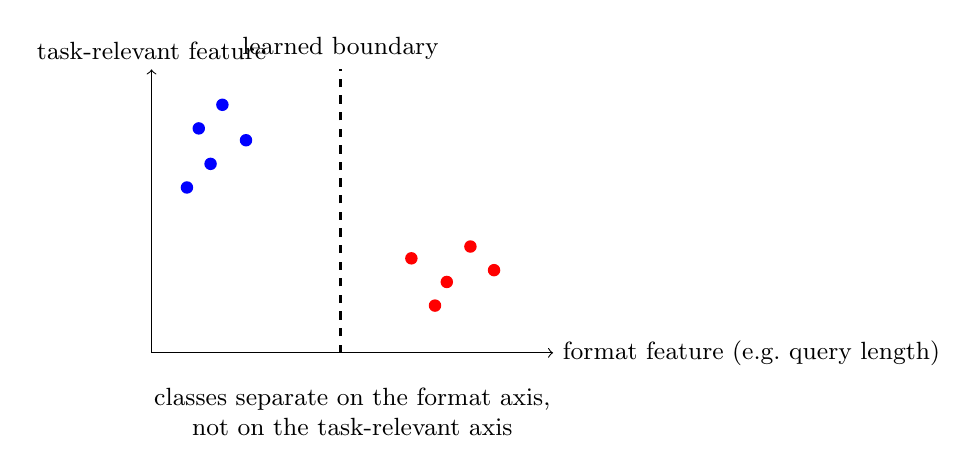
\begin{tikzpicture}[scale=1.5]
  % Axes
  \draw[->] (0,0) -- (3.4,0) node[right, font=\small] {format feature (e.g.\ query length)};
  \draw[->] (0,0) -- (0,2.4) node[above, font=\small] {task-relevant feature};
  % Class A points
  \foreach \p in {(0.4,1.9),(0.6,2.1),(0.5,1.6),(0.8,1.8),(0.3,1.4)} \fill[blue] \p circle (1.5pt);
  % Class B points
  \foreach \p in {(2.5,0.6),(2.7,0.9),(2.4,0.4),(2.9,0.7),(2.2,0.8)} \fill[red] \p circle (1.5pt);
  % Separating line (follows format axis)
  \draw[thick, dashed] (1.6,0) -- (1.6,2.4) node[above, font=\small] {learned boundary};
  \node[font=\small, align=center] at (1.7,-0.5) {classes separate on the format axis,\\ not on the task-relevant axis};
\end{tikzpicture}
\caption{The format-confound failure mode. The two classes are perfectly separable, but the separating direction tracks a confounded surface feature rather than the property of interest. Residualizing the surface feature collapses the separation, as \textcite{sahoo2026linear} demonstrate. (Preliminary figure.)}
\label{fig:confound}
\end{figure}


These critiques motivate design constraints for later measurements.
Template matched queries keep the target tool as the only systematic difference between classes, position balanced extraction keeps list position out of the signal, and permutation baselines follow the control task tradition.
Reporting both raw separability and separability after residualizing surface features separates what is present from what adds predictive power.

\subsection{The Linear Representation Hypothesis}
\label{sec:linearrep}

Probing asks whether a property can be read out of a hidden state.
A stronger claim is that high-level concepts are represented as directions, meaning that varying the concept corresponds to moving along a fixed direction in the representation space.
This is the linear representation hypothesis, and \textcite{park2024linear} gave it a formal treatment.
They distinguish three senses of linear representation that had been used interchangeably: a concept as a subspace shared by counterfactual pairs, a concept as something measurable by a linear probe, and a concept as something changeable by adding a steering vector.
Using a counterfactual formalization, they prove that the measurement and intervention notions connect to representations in the unembedding and embedding spaces respectively, and that a suitable inner product unifies the two.
\Cref{fig:conceptdirection} illustrates the idea.

\begin{figure}[htbp]
\centering
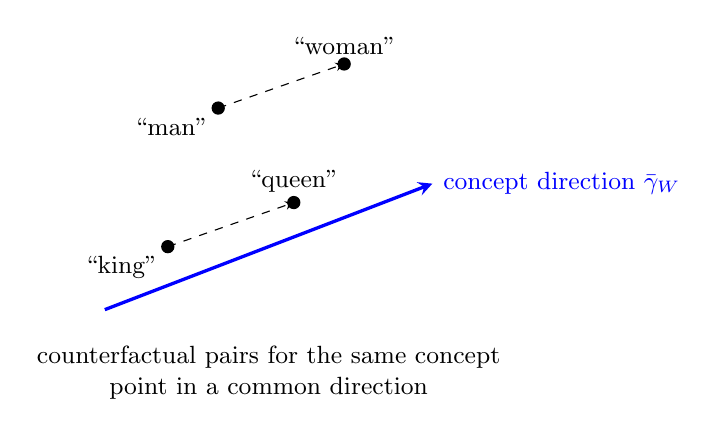
\begin{tikzpicture}[scale=1.6, >=stealth]
  % Concept direction
  \draw[->, very thick, blue] (0,0) -- (2.6,1.0) node[right, font=\small] {concept direction $\bar{\gamma}_W$};
  % Counterfactual pairs
  \fill (0.5,0.5) circle (1.5pt) node[below left, font=\small] {``king''};
  \fill (1.5,0.85) circle (1.5pt) node[above, font=\small] {``queen''};
  \draw[->, dashed] (0.5,0.5) -- (1.5,0.85);
  \fill (0.9,1.6) circle (1.5pt) node[below left, font=\small] {``man''};
  \fill (1.9,1.95) circle (1.5pt) node[above, font=\small] {``woman''};
  \draw[->, dashed] (0.9,1.6) -- (1.9,1.95);
  \node[font=\small, align=center] at (1.3,-0.5) {counterfactual pairs for the same concept\\ point in a common direction};
\end{tikzpicture}
\caption{The subspace notion of the linear representation hypothesis. Differences between counterfactual pairs for one concept, such as $\gamma(\text{queen}) - \gamma(\text{king})$ and $\gamma(\text{woman}) - \gamma(\text{man})$, align with a common direction $\bar{\gamma}_W$ \cite{park2024linear}. (Preliminary figure.)}
\label{fig:conceptdirection}
\end{figure}


The empirical evidence for linear concept directions is broad.
\textcite{marks2024geometry} showed that true and false statements are linearly separable in the hidden states of LLaMA-2 models, that simple difference-in-mean directions generalize across datasets, and that intervening along those directions flips the model's judgment of truth.
\textcite{todd2024function} found that in-context learning tasks are carried by function vectors, directions extracted from a small set of attention heads in middle layers, and that adding a function vector to a prompt that never demonstrates the task causes the model to execute the task anyway.
Notably, their residual-stream formulation of the hidden state, $\mathbf{h}_\ell = \mathbf{h}_{\ell-1} + \mathbf{m}_\ell + \sum_j \mathbf{a}_{\ell j}$ as a sum of attention-head and feed-forward contributions, is the same framing used in \cref{sec:transformer}.
\\

A direct antecedent for tool identity is \textcite{wu2026linearly}, who showed that tool identity is a linear direction.
For each tool, they average the residual-stream hidden states over a few example queries, and the normalized difference between two tool means is a direction that, when added during generation, switches the model's selection from one tool to the other.
The same per-tool means support a training-free readout, where the tool whose mean is closest to the current hidden state in cosine similarity is usually the tool the model is about to call.
\Cref{fig:toolgeometry} shows the geometry for a pair of tools.

\begin{figure}[htbp]
\centering
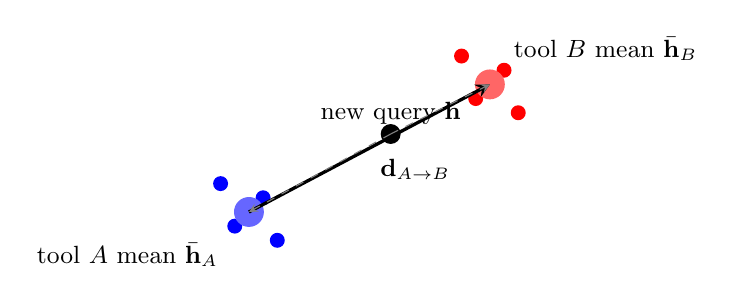
\begin{tikzpicture}[scale=1.8, >=stealth]
  % Tool A cluster
  \foreach \p in {(0.4,0.4),(0.6,0.6),(0.3,0.7),(0.7,0.3),(0.5,0.5)} \fill[blue] \p circle (1.5pt);
  \fill[blue!60] (0.5,0.5) circle (3pt);
  \node[font=\small, below left] at (0.35,0.35) {tool $A$ mean $\bar{\mathbf{h}}_A$};
  % Tool B cluster
  \foreach \p in {(2.1,1.3),(2.3,1.5),(2.0,1.6),(2.4,1.2),(2.2,1.4)} \fill[red] \p circle (1.5pt);
  \fill[red!60] (2.2,1.4) circle (3pt);
  \node[font=\small, above right] at (2.3,1.5) {tool $B$ mean $\bar{\mathbf{h}}_B$};
  % Mean-difference direction
  \draw[->, very thick] (0.5,0.5) -- (2.2,1.4) node[midway, below right, font=\small] {$\mathbf{d}_{A \to B}$};
  % Current query point, near boundary
  \fill[black] (1.5,1.05) circle (2pt) node[above, font=\small] {new query $\mathbf{h}$};
  \draw[->, dashed, gray] (1.5,1.05) -- (0.5,0.5);
  \draw[->, dashed, gray] (1.5,1.05) -- (2.2,1.4);
\end{tikzpicture}
\caption{The geometry of a tool pair. Each tool's hidden states cluster around a mean, the mean-difference direction $\mathbf{d}_{A \to B}$ points from one center to the other, and a new query is read off by its cosine distance to the two means \cite{wu2026linearly}. Pairs differ in how cleanly they separate and how close new queries fall to the boundary. (Preliminary figure.)}
\label{fig:toolgeometry}
\end{figure}


Their results establish that tool identity is linearly represented.
They do not establish whether the degree of separation between two tools predicts how often the model confuses them.

\subsection{Mechanistic Interpretability}
\label{sec:mechinterp}

Mechanistic interpretability is the research program of reverse-engineering the computations a neural network performs, rather than only measuring what information its representations contain.
The central obstacle is superposition.
\textcite{elhage2022superposition} showed that models routinely pack more features than they have neurons, storing several concepts in overlapping directions, so that individual neurons rarely correspond to clean, human-interpretable features.
One response is to analyze directions rather than neurons.
Another is sparse autoencoders, which decompose hidden states into a larger set of sparsely active features \cite{cunningham2023sae}.
\\

Attention heads are the other major unit of analysis.
\textcite{olsson2022induction} identified induction heads, attention heads that complete repeated patterns by finding earlier occurrences of the current token and copying what followed them, and gave evidence that such heads underlie much of in-context learning.
In the tool-selection setting, \textcite{wu2026linearly} found that a small number of middle-layer attention heads carry most of the causal effect on which tool is chosen, and \textcite{chen2026looking} showed that the model's attention to the correct tool's specification usually survives even when the final choice is wrong.
\\

Correlational claims in this literature are routinely backed by causal intervention.
The standard method is activation patching, grounded in causal mediation analysis \cite{vig2020causal}.
The idea is to run the model on a clean input, run it again on a corrupted input, and replace one internal component's activation in the corrupted run with its value from the clean run.
The amount by which the model's output recovers measures the causal contribution of that component.
\Cref{fig:patching} shows the procedure.

\begin{figure}[htbp]
\centering
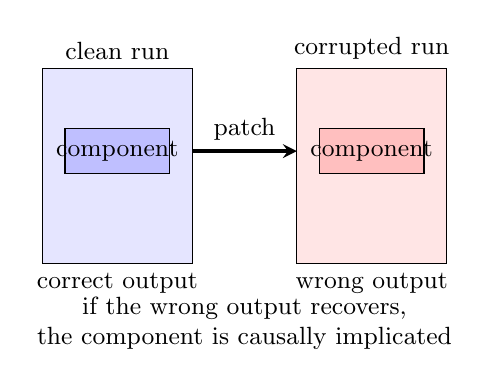
\begin{tikzpicture}[scale=0.95, >=stealth]
  % Clean run
  \draw[fill=blue!10] (0,0) rectangle (2.0,2.6);
  \node[font=\small, above] at (1.0,2.6) {clean run};
  \draw[fill=blue!25] (0.3,1.2) rectangle (1.7,1.8) node[midway, font=\small] {component};
  \node[font=\small, below] at (1.0,0) {correct output};
  % Corrupted run
  \draw[fill=red!10] (3.4,0) rectangle (5.4,2.6);
  \node[font=\small, above] at (4.4,2.6) {corrupted run};
  \draw[fill=red!25] (3.7,1.2) rectangle (5.1,1.8) node[midway, font=\small] {component};
  \node[font=\small, below] at (4.4,0) {wrong output};
  % Patch arrow
  \draw[->, very thick] (2.0,1.5) -- (3.4,1.5) node[midway, above, font=\small] {patch};
  % Recovery note
  \node[font=\small, align=center] at (2.7,-0.8) {if the wrong output recovers,\\ the component is causally implicated};
\end{tikzpicture}
\caption{Activation patching. A component's activation from the clean run is inserted into the corrupted run. The degree to which the correct output recovers measures the component's causal contribution \cite{vig2020causal}. (Preliminary figure.)}
\label{fig:patching}
\end{figure}

\textcite{todd2024function} used exactly this procedure to identify the attention heads that transport function vectors, and \textcite{sun2026dependency} used it to show that the tool-call dependency signal propagates through the residual stream rather than sitting still.
Separability is a correlational quantity.
The intervention literature is what licenses reading it as a property of the decision process rather than a geometric curiosity.

\subsection{Measuring Representational Similarity}
\label{sec:repsim}

The final ingredient is a family of methods for comparing sets of representations.
The oldest comes from neuroscience.
\textcite{kriegeskorte2008rsa} introduced representational similarity analysis, in which a representation is characterized not by the patterns themselves but by the matrix of pairwise dissimilarities between them.
Two representational spaces are then compared by correlating their dissimilarity matrices, which abstracts away from any particular choice of coordinates.
\textcite{raghu2017svcca} took a complementary approach with SVCCA, which compares two layers by finding the directions of maximal correlation between them after a dimensionality reduction step.\footnote{RSA and SVCCA answer the question of whether two representational spaces carry the same information in some form. A more targeted question is whether two classes can be told apart at the point of decision. The measures are listed here for completeness, since a reader from neuroscience or vision will expect them to be acknowledged.}
\\

A simpler task tied measure is a two class probe.
For a pair of tools, hidden states of queries targeting each tool are collected and a two-class linear probe is trained to separate them.
The cross-validated accuracy of that probe is a direct separability measure, because it answers whether the two tools occupy distinguishable regions at the point where the model makes its choice.
Two descriptive quantities accompany it.
The centroid cosine distance applies \cref{eq:cosine} to the two class means, and the between-to-within scatter ratio compares how far apart the class means are to how spread out each class is:

\begin{equation}
S(A, B) = \frac{\lVert \bar{\mathbf{h}}_A - \bar{\mathbf{h}}_B \rVert^2}{\frac{1}{2}\left( \sigma_A^2 + \sigma_B^2 \right)}
\label{eq:scatter}
\end{equation}

where $\sigma_A^2$ and $\sigma_B^2$ are the mean squared distances of the hidden states to their own class mean.
The scatter ratio is the classical Fisher criterion, and it captures the intuition that two groups are well separated when their centers are far apart relative to how much each group spreads around its own center.
\Cref{fig:scatter} shows the two factors that determine the ratio.

\begin{figure}[htbp]
\centering
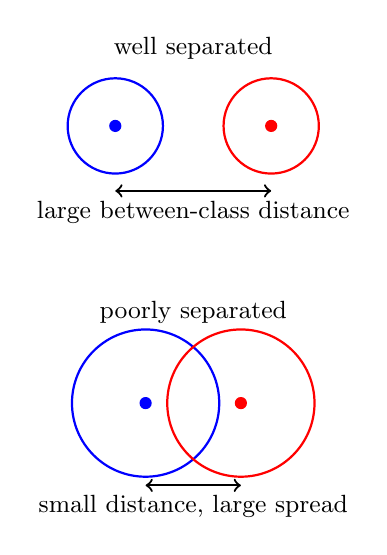
\begin{tikzpicture}[scale=1.1]
  % Top row: far means
  \begin{scope}
    \draw[blue, thick] (0.8,1.0) circle (0.55);
    \draw[red, thick] (2.6,1.0) circle (0.55);
    \fill[blue] (0.8,1.0) circle (2pt);
    \fill[red] (2.6,1.0) circle (2pt);
    \draw[<->, thick] (0.8,0.25) -- (2.6,0.25) node[midway, below, font=\small] {large between-class distance};
    \node[font=\small] at (1.7,1.9) {well separated};
  \end{scope}
  % Bottom row: close means, wide spread
  \begin{scope}[yshift=-3.2cm]
    \draw[blue, thick] (1.15,1.0) circle (0.85);
    \draw[red, thick] (2.25,1.0) circle (0.85);
    \fill[blue] (1.15,1.0) circle (2pt);
    \fill[red] (2.25,1.0) circle (2pt);
    \draw[<->, thick] (1.15,0.05) -- (2.25,0.05) node[midway, below, font=\small] {small distance, large spread};
    \node[font=\small] at (1.7,2.05) {poorly separated};
  \end{scope}
\end{tikzpicture}
\caption{The two factors in the scatter ratio of \Cref{eq:scatter}. Top: class means far apart relative to within-class spread gives a large ratio. Bottom: class means close together relative to spread gives a small ratio. (Preliminary figure.)}
\label{fig:scatter}
\end{figure}


These pairwise geometric quantities are computed once per tool pair.
Cheap baselines are string similarity for lexical overlap, sentence embedding similarity for semantic overlap under an off the shelf encoder, and the output side pair margin for the gap in probability mass.
If internal separability cannot beat these, the practical conclusion is that internals are unnecessary for this task.

\section{Related Work}

This section reviews the literature on tool selection in language model agents, organized around the chain of evidence that leads to this thesis.
We first establish that tool selection is fragile and driven by surface features of tool specifications.
We then examine work that reads tool-related information from the internal representations of models.
Next we review the conflicting evidence on which specification component drives selection errors.
We close with the methodological controls that probing experiments require, and state the gap that the present work addresses.

\subsection{Tool Selection is Fragile}

A growing body of work shows that tool selection in LLM agents is sensitive to surface features of tool specifications rather than their actual functionality.
\textcite{sneh2025tooltweak} introduced ToolTweak, an adversarial attack that iteratively rewrites a tool's name and description to increase its selection rate.
The attack follows a PAIR-inspired loop, where an attacker model proposes new metadata, the victim model is evaluated on a fixed set of queries, and the measured selection rate feeds back into the next proposal. Unlike PAIR there is no separate judge model.
Across six models, ToolTweak raises selection rates from a baseline near 20\% to as high as 81.6\% on DeepSeek, with substantial transferability between open-source and closed-source models.
Two findings from that work matter directly for this thesis.
First, on the Berkeley Function Calling Leaderboard, two identical tools differing only by a numeric suffix received drastically different selection rates, which the authors interpret as ordinality in names implicitly signaling a ranking.
Second, parameter schema complexity affected how usable a tool was to the model, but the authors explicitly left a controlled study of schema effects to future work.
\\

\textcite{blankenstein2025biasbusters} conducted a systematic study of tool-selection bias, evaluating seven LLMs on a benchmark of 10 clusters, each containing 5 functionally equivalent APIs and 100 queries.
They quantify bias as the total variation distance between the empirical selection distribution and the uniform distribution, measured both per API and per list position, and find that all tested models exhibit substantial bias, with combined metrics around 0.3 to 0.4.
Their perturbation experiments establish a clear hierarchy among specification components.
Scrambling descriptions and parameters together produces the largest reliable shift in selection (mean TV distance 0.450 for Gemini), scrambling the description of the most-selected tool follows at 0.419, and swapping descriptions between tools still meaningfully steers choices at 0.338.
Name-only perturbations are smaller and have higher variance, and parameter-only perturbations are the least impactful.
Their feature analysis identifies semantic similarity between query and description as the strongest single predictor of selection, though a linear model over seven features explains less than 40\% of variance.
They further show that biased continued pre-training on 3.5M tokens saturated with one endpoint raises that endpoint's selection share from 0.6\% to 12.2\%, demonstrating that pre-training exposure plants durable but not dominant preferences.
\\

\textcite{lu2024toolsandbox} built ToolSandbox, a stateful, conversational tool-use benchmark, and included controlled ablations over specification components that are directly relevant here.
For GPT-4o, scrambling tool descriptions lowers the average task score from 73.0 to 69.3, while scrambling tool names leaves it nearly unchanged at 72.4. Scrambling argument types has an intermediate effect at 71.9, while scrambling argument descriptions leaves the average unchanged at 73.0.
The pattern is model-dependent, since GPT-4 actually improves under name scrambling, from 64.3 to 69.7, which suggests different models rely on different components.
Their ablations vary one component at a time and measure aggregate task accuracy, so they cannot reveal how components interact or which pairs of tools become confusable as a result.
\\

Together, these studies establish that selection behavior is driven by surface metadata, that the effect is reproducible across model families, and that the influence of the three specification components is not uniform.
Such sensitivity to surface features is not unique to tool selection. Instruction-tuned models exhibit emergent cognitive biases more broadly, including biases triggered by the phrasing of instructions themselves \cite{itzhak2024instructed}.
That finding matters here because a tool specification is itself a piece of instruction text. Wording choices in the name and description may therefore bias selection in the same way that instruction phrasing biases answers.
However, all three measure selection share or task accuracy aggregated over a tool set.
None of them asks whether a specific pair of tools is confused with each other, at what rate, or why.
A tool can be systematically over-selected without being confusable with any particular sibling, and preference bias of this kind is a different quantity from pairwise confusability.

\subsection{Internal Representations of Tool Selection}

A separate line of work asks what the model knows internally when it selects a tool.
\textcite{sun2026when2tool} probed pre-generation hidden states to predict whether a tool call is necessary at all.
Their benchmark, When2Tool, spans 18 environments in three categories of tool necessity, with controlled difficulty levels that create a clean decision boundary between tasks the model can and cannot solve directly.
A logistic regression probe on the last-input-token hidden state, with all layers concatenated, predicts tool necessity with AUROC 0.89 to 0.96 across six models from the Qwen3 and Llama families.
The signal persists even in models whose explicit reasoning about tool necessity collapses behaviorally, which shows that representation-level knowledge exists independently of the model's ability to act on it during generation.
Their Probe\&Prefill method reads the probe output and prefills a steering sentence, reducing tool calls by 48\% at a cost of 1.7\% accuracy.
The probe target in this work is binary necessity, meaning whether to call a tool at all, not the identity of the tool being called.
\\

The closest prior work to this thesis is \textcite{wu2026linearly}, who showed that the choice of tool is carried by a single direction in activation space, with one direction per pair of tools.
Their method computes mean residual-stream activations per tool from two or three queries, takes the normalized difference between two tool means as a steering direction, and adds it at the second-to-last layer during generation.
This intervention switches the selected tool at 83 to 100\% accuracy on 4B and larger instruction-tuned models across Gemma 3, Qwen 3, and Llama 3.1 families, on both a synthetic 15-tool benchmark and the real-API $\tau$-bench airline benchmark.
A multinomial probe trained on pre-emission residual states reads which tool the model will call at 61 to 89\% top-1 accuracy even within a single domain of 14 airline tools, ruling out the explanation that the probe merely detects topic.
Most relevant to our central question, they report that queries where the model is unsure between two tools, measured by a small cosine gap between the top-1 and top-2 tool means, fail 21 times more often than queries where the model is confident.
\\

Three properties of their design define the space this thesis occupies.
First, their uncertainty analysis is per query and pooled across queries into quartiles.
They never compute a separability score for a specific pair of tools, and they never regress a pair's empirical confusion rate on its separability.
Second, they test no surface-similarity baselines, so it remains unknown whether internal geometry adds predictive power beyond what string overlap or sentence-embedding similarity of the specifications already provides.
Third, their steering fails exactly where confusion is worst, achieving 0\% switch rate on a set of near-synonymous sports APIs, which they attribute to the model being unable to distinguish the tools at all.
That failure mode is precisely the phenomenon this thesis aims to measure and predict.
\\

Three further papers probe tool-related information from hidden states without touching tool identity.
\textcite{healy2026internal} detect tool-calling hallucinations by training a small classifier on final-layer hidden states taken at three positions of the generated call, namely the function-name token, the mean-pooled argument tokens, and the closing delimiter.
Their framework achieves up to 86.4\% accuracy in distinguishing correct from hallucinated calls on the Glaive function-calling dataset, with labels generated automatically by masking the reference call and comparing the model's re-prediction against it.
Their classification target is a binary correct-versus-hallucinated label, so the probe learns that something went wrong without decoding which tool was involved or which alternative it was confused with.
\textcite{sun2026dependency} probe the residual stream of Qwen3-32B for a different structure, the dependency edges between sequential tool calls in an agent trajectory, using a logistic edge probe over concatenated residual vectors of call pairs.
Their signal tracks the abstract topology of the call graph rather than identifier values, and it concerns the temporal structure of a call sequence, not competition between candidate tools.
\\

\textcite{chen2026looking} takes an attention-based view.
Measuring per-segment attention to each tool definition in the prompt, they find that on real BFCL failures the model attends most to the correct tool 80\% of the time, against 21\% chance, and still selects the wrong tool.
Repairing the prompt by reordering or duplicating the correct tool recovers at most 23\% of failures, while readout-side interventions recover 59 to 91\%, localizing the failure at the decision readout rather than at input encoding.
Their attention margin between the correct tool and the distractors predicts per-query failure competitively with a trained hidden-state probe on real benchmarks, and a causal attention-logit bias raises the probability of the correct tool monotonically.
Like the other work in this subsection, their unit of analysis is the individual query, and the attention margin is a per-query confidence signal rather than a property of a tool pair.
\\

Taken together, this literature establishes that tool-related information is linearly present in hidden states, that the chosen tool is readable and steerable per pair, and that per-query uncertainty predicts per-query failure.
What none of it provides is a measurement at the level of the tool pair: whether the representational distance between two specific tools, computed once from their specifications, predicts how often the model confuses them across queries, and whether that prediction beats cheap surface baselines.

\subsection{Component Attribution and Conflicting Evidence}

If pairwise confusion is to be reduced by rewriting specifications, the practical question is which component of the specification to rewrite.
The published evidence on this question conflicts.
On the side of names, \textcite{sneh2025tooltweak} found that identical tools differing only by a numeric suffix receive very different selection rates.
On the side of descriptions, \textcite{faghih2025gaming} report that carefully edited tool descriptions can increase a tool's usage by more than ten times on GPT-4.1 and Qwen2.5-7B.
In the same direction, \textcite{blankenstein2025biasbusters} found name-only perturbations small and high-variance while description semantics were the primary discrimination cue, and the ToolSandbox ablations \cite{lu2024toolsandbox} show description scrambling costing GPT-4o more than six times as much accuracy as name scrambling.
None of these studies estimates an interaction between components, and none of them measures confusion between a specific pair of sibling tools as the outcome.
\\

The parameter schema has received less attention in the selection literature, but one mechanistic result suggests it deserves equal standing.
\textcite{liu2026structural} identified structural alignment bias, the tendency of models to invoke a tool whenever the attributes in the query can be validly assigned to its parameters, even when the tool is semantically irrelevant to the goal.
On their SABEval dataset, which decouples structural alignment from semantic relevance through a polymorphism-inspired construction of sibling tools, tool invocation rates on irrelevant tools rise from under 0.2\% under random pairing to 41.9\% under structural alignment, and further to 90.4\% as the number of aligned attribute-parameter assignments grows.
Their contrastive attention attribution method reveals two competing pathways inside the model, one performing semantic checking and one performing structural matching, and the relative strength of the two pathways drives the invocation decision.
This result motivates treating the schema as a first-class factor in our attribution experiment, since a schema that admits a valid assignment may pull the model toward a sibling tool even when the name and description point elsewhere.
\\

\textcite{anand2026canary} take a behavioral diagnostic approach to the same family of questions with canary tools, planted probe tools engineered so that selecting them exposes a specific reasoning weakness.
Their six-type taxonomy covers semantic decoys, parameter traps, capability mirages, prerequisite blindness, temporal decoys, and granularity traps, and their evaluation over eight models and 8,640 runs shows that susceptibility varies roughly 36-fold across models and does not track capability tier.
Their work demonstrates the value of controlled, diagnostic tool design and provides a taxonomy of selection weaknesses, but it is purely behavioral, with no internal measurement and no attribution of confusion to specification components.
\\

The conflicting evidence, the one-factor-at-a-time designs, and the absence of a pairwise confusion outcome together motivate our factorial attribution experiment.
We cross the three components, name, description, and schema, in a full factorial design over matched sibling pairs, which allows interaction terms to be estimated directly.
Our expectation, stated in advance, is that no single component dominates, and that name overlap matters most when descriptions leave the boundary between two siblings unstated, while description quality matters most when names are already distinct.

\subsection{Methodological Controls for Probing}

Probing hidden states is an established but easily misused technique, and the design of our separability measurement follows directly from its documented failure modes.
\textcite{alain2016understanding} introduced linear classifier probes as a measurement instrument for intermediate layers, showing that the linear separability of features increases monotonically with depth and framing probes as thermometers that measure a property of the model without influencing it.
\textcite{belinkov2022probing} reviewed the framework critically, emphasizing that high probe accuracy alone is weak evidence, since a sufficiently expressive probe can memorize a mapping that the model never uses, and that control tasks and comparisons against baselines are necessary for interpretation.
\\

As described in \cref{sec:probing}, \textcite{sahoo2026linear} show how format confounds can drive probe accuracy to chance once residualized.
Applied to our setting, a probe that separates queries targeting tool A from queries targeting tool B may have learned stylistic register, query length, or lexical overlap with the tool name rather than tool identity.
\\

These results shape our measurement design in four concrete ways.
First, all queries in the separability experiment share a single template frame with a varying slot fill, so the only systematic difference between the two classes is the target tool.
Second, extraction is balanced across tool-list positions, since activations are position-sensitive and an unbalanced design would let the probe learn list position.
Third, we report both raw separability and separability residualized against query length, token count, and lexical overlap with the tool name, and we state explicitly what each quantity licenses.
Fourth, every probe result is accompanied by a permutation baseline with shuffled labels, following the control-task tradition that \textcite{hewitt2019control} describe.

\subsection{The Gap}

The literature establishes four premises.
Surface metadata causally drives selection \cite{sneh2025tooltweak}.
Selection bias is reproducible across model families \cite{blankenstein2025biasbusters}.
Tool-related decisions, including both necessity and identity, are linearly decodable from hidden states \cite{sun2026when2tool,wu2026linearly}.
Parameter schemas drive invocation through a structural-matching pathway that operates independently of semantic relevance \cite{liu2026structural}.
\\

To our knowledge, what is missing is a measurement that connects these premises at the level of the tool pair.
No prior work computes a separability statistic for a specific pair of tools and tests whether it predicts that pair's empirical confusion rate.
No prior work compares an internal separability signal against surface-similarity and sentence-embedding baselines to establish whether internals add predictive power at all.
No prior work attributes pairwise separability to the name, description, and schema components in a factorial design that can detect their interaction.
And no prior work tests whether an attribution of this kind is actionable, by measuring whether edits guided by the attributed cause reduce confusion against a sham edit of equal effort.
These four gaps define the four experiments of this thesis.
